\documentclass[compress]{beamer}

\usepackage[nofonts]{ctex}
\setCJKmainfont[ItalicFont={Kaiti SC}]{Kaiti SC}%
%\setCJKmainfont[ItalicFont={AR PL KaitiM GB}]{AR PL KaitiM GB}%
%\setCJKsansfont{WenQuanYi Zen Hei}% 文泉驿的黑体

\mode<beamer>
{
    \setbeamercovered{transparent}

    \useinnertheme{rounded}
    %\useoutertheme{miniframes}
    \useoutertheme{split}
    %\usecolortheme{orchid}
    %\usecolortheme{whale}
    %\usecolortheme{lily}
    \usecolortheme{rose}
    \usecolortheme{seahorse}
	\expandafter\def\expandafter\insertshorttitle\expandafter{%
	\insertshorttitle\hfill%
	\insertframenumber\,/\,\inserttotalframenumber}
}

\mode<handout>
{
	\usetheme{default}
	\usepackage{pgfpages}
	\pgfpagesuselayout{4 on 1}[a4paper,landscape,border shrink=5mm]
}


\usepackage{amsmath,latexsym,amssymb,amsfonts,amsbsy}
\usepackage{graphicx}
\usepackage{hyperref}
\usepackage{listings}
\usepackage{fancyvrb}
\fvset{frame=single,fontsize=\small}

\newcommand{\romannumber}[1]{{\textrm{\uppercase\expandafter{\romannumeral
#1}}}}
\setbeamercolor{dblue}{fg=white,bg=blue!40!black} % for beamercolorbox
\newenvironment{pblock}{\begin{beamercolorbox}[rounded=true,
                          shadow=true]{dblue}}{\end{beamercolorbox}}

\graphicspath{{figure/}}

\lstset{
	basicstyle=\footnotesize\ttfamily, % print whole listing footnotesize
	keywordstyle=\ttfamily\color{black}\bfseries\footnotesize, 
	identifierstyle=\ttfamily\color{blue}\footnotesize, 
	commentstyle=\itshape\ttfamily\footnotesize, 
	stringstyle=\ttfamily\footnotesize,
	frame=single, 
	numbers=left, numberstyle=\tiny,
	stepnumber=1, numbersep=10pt,
	showtabs=false, tabsize=4,
	showstringspaces=false,
	breaklines=true, breakatwhitespace=true,
	language=[ISO]C++
}   


%%%%%%%%%%%%%%%%%%%%%%%%%%%%%%%%%%%%%%%%%%%%%%%%%%%%%%%%%%%%%%%%%
%    body                                                       %
%%%%%%%%%%%%%%%%%%%%%%%%%%%%%%%%%%%%%%%%%%%%%%%%%%%%%%%%%%%%%%%%%


\begin{document}

\AtBeginSection[]
{ 
    \begin{frame}<beamer> 
		\frametitle{内容提要} 
		\tableofcontents[currentsection,currentsubsection] 
	\end{frame} 
} 
					
\title{Linux开发工具}

\author[\href{http://c.pku.edu.cn/}{http://c.pku.edu.cn/}]
{曹东刚\\\href{mailto:caodg@sei.pku.edu.cn}{caodg@sei.pku.edu.cn}}

\institute{Linux程序设计环境 \\
\href{http://c.pku.edu.cn/}{
http://c.pku.edu.cn/}}

\date{}

\titlegraphic{
\includegraphics[height=0.17\textwidth]{Overlays/logo.pdf}}

\begin{frame}
	\titlepage
\end{frame}

\begin{frame}
\frametitle{Unix开发模型}
\setlength{\unitlength}{1cm}
\begin{picture}(13,1.5)
\put(0,0){\framebox(2,1){编辑}} \put(4,0){\framebox(2,1){编译}}
\put(8,0){\framebox(2,1){调试}} \thicklines
\put(2,0.5){\vector(1,0){2}} \put(6,0.5){\vector(1,0){2}}
\end{picture}

\begin{itemize}
\item 大量久经考验的高质量专业工具
\item cmdline vs IDE
\item 让工具自动完成脏活累活
\item 编辑器: vi vs emacs
\end{itemize}

\end{frame}

\begin{frame}
	\frametitle{binutils}
	\begin{itemize}
	\item size
	\item strings
	\item ranlib
	\item nm
	\item strip
	\item as
	\item ld
	\item objdump
	\end{itemize}
\end{frame}


\section{静态检查}

\subsection{lint}

\begin{frame}
    \frametitle{静态检查工具}
    \begin{itemize}
        \item lint: 代码分析检查工具
            \begin{itemize}
                \item 很多功能被现代编译器取代
            \end{itemize}
        \item cppcheck
        \item findbugs等语言特定工具
    \end{itemize}
\end{frame}

\begin{frame}[fragile]
    \frametitle{cppcheck}
\begin{lstlisting}
void tryit()
{
    int a[4];
    int z = 4 + 1;

    for (int n = 0; n < z; n++) {
        a[n] = n;
    }
}
\end{lstlisting}

\end{frame}

\begin{frame}[fragile]
\frametitle{cppcheck (cont.)}
\begin{verbatim}
$ cppcheck --enable=all -v z.c
caodg@mars:~/ex$ cppcheck --enable=all -v z.c
Checking z.c...
[z.c:3]: (style) Variable 'a' is assigned a value
  that is never used
[z.c:8]: (error) Buffer access out-of-bounds: a
Checking usage of global functions..
[z.c:1]: (style) The function 'tryit' is never used
\end{verbatim}
\end{frame}


\subsection{gcc}

\begin{frame}
\frametitle{gcc历史}

\begin{itemize}

\item 1980s中期, RMS为FSF的GNU项目开发: Gnu C Compiler
\item 1987年5月, gcc 1.0 发布
\item 1992年, gcc 2.0发布, 支持C++
\item 1997年, Cygnus EGCS (Experimental/Enhanced GNU Compiler System)项目
\item 1999年, EGCS委员会成为FSF指定的gcc官方维护者 Gnu Compiler Collection
\item 2001年, gcc 3.0 发布, 支持 c++, Java, objective-c等
\end{itemize}
\end{frame}

\begin{frame}
\frametitle{支持语言}

\begin{itemize}

\item Ada (GCC for Ada aka GNAT)
\item C
\item C++ (GCC for C++ aka G++)
\item Fortran (GCC for Fortran aka GFortran)
\item Java (GCC for Java aka GCJ)
\item Objective-C
\item 以及Pascal, Modula-2, Modula-3, Mercury, VHDL, PL/I, Objective-C++等
\end{itemize}

\end{frame}

\begin{frame}
\frametitle{gcc特征}

\begin{itemize}
\item 可移植
\item 支持交叉编译
\item 有多种语言前端
\item 模块化结构, 易扩展
\item 免费
\end{itemize}
\end{frame}

\begin{frame}
\frametitle{gcc工作过程}

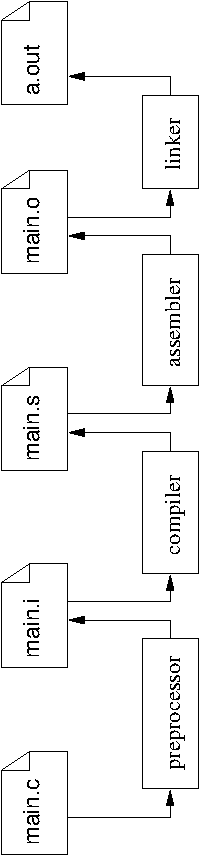
\includegraphics[angle=-90,width=1.0\hsize]{gcc_process.pdf}\\

\begin{itemize}
\item 预处理, e.g., \emph{cpp}
\item 编译, e.g., \emph{cc}
\item 汇编, e.g., \emph{as}
\item 链接, e.g., \emph{ld}
\end{itemize}

\end{frame}

\begin{frame}
\frametitle{前端与后端}

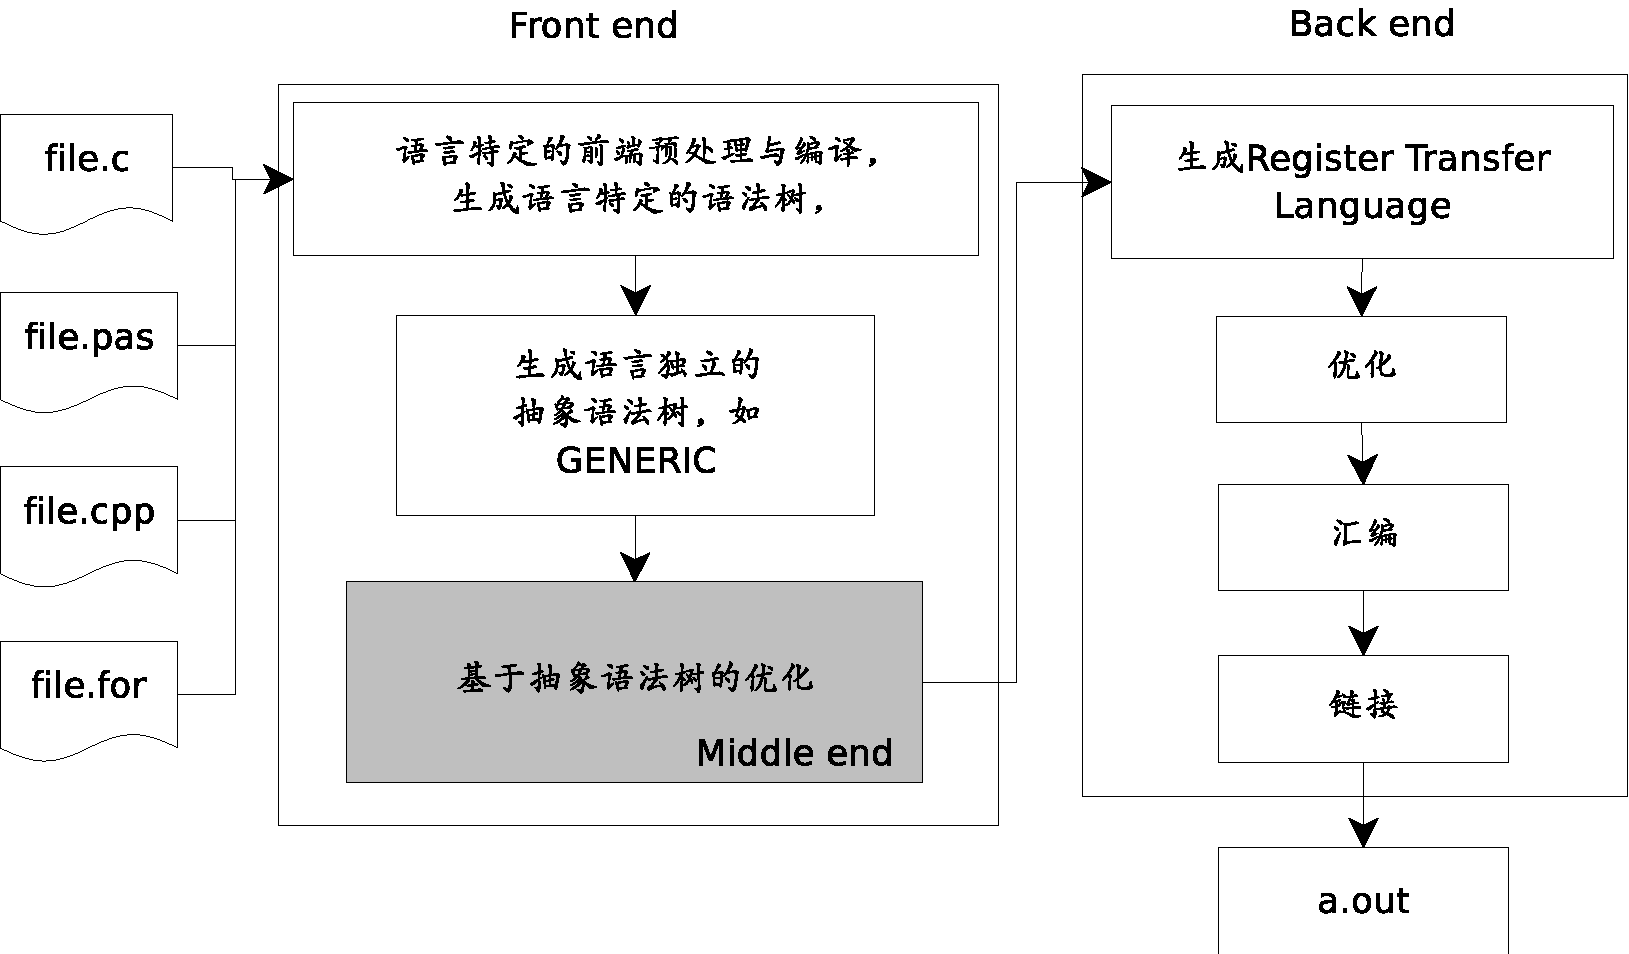
\includegraphics[width=1.0\hsize]{gcc_twophase.pdf}\\

\end{frame}

\begin{frame}[fragile]
\frametitle{编译一个C程序---hello.c}

\begin{lstlisting}
#include <stdio.h>
int
main (void)
{
    printf ("Hello, world!\n");
    return 0;
}
\end{lstlisting}

\verb~$ gcc -Wall hello.c -o hello~

\end{frame}

\begin{frame}[fragile]
\frametitle{检查错误---bad.c}

\begin{lstlisting}
#include <stdio.h>
int
main (void)
{
    printf ("Two plus two is %f\n", 4);
    return 0;
}
\end{lstlisting}

\footnotesize
\begin{verbatim}
$ gcc -Wall bad.c
bad.c: In function ‘main’:
bad.c:5:5: warning: format ‘%f’ expects argument of type 
‘double’, but argument 2 has type ‘int’ [-Wformat]
\end{verbatim}
\end{frame}


\begin{frame}[fragile]
\frametitle{编译多个文件: 将Hello World程序分开 --1}\label{multifile}
\begin{lstlisting}
#include "hello.h"
int main (void)
{
    hello ("world");
    return 0;
}
\end{lstlisting}

\end{frame}

\begin{frame}[fragile]
\frametitle{编译多个文件: 将Hello World程序分开 --2}
\begin{lstlisting}
#include <stdio.h>
#include "hello.h"
void hello (const char * name)
{
    printf ("Hello, %s!\n", name);
}
\end{lstlisting}
\begin{verbatim}
$ gcc -Wall main.c hello.c -o newhello
\end{verbatim}
\end{frame}


\begin{frame}
\frametitle{单独编译每个文件---1}

\begin{itemize}
\item 将一个大文件分成若干小文件
\item 只编译改动的源文件
\item 两阶段编译过程
    \begin{itemize}
    \item 编译生成目标文件 file.o
    \item 链接生成可执行文件
    \end{itemize}
\end{itemize}
\end{frame}

\begin{frame}[fragile]
\frametitle{单独编译每个文件---2}

\begin{itemize}
\item 链接顺序: 包含函数定义的目标文件声明在调用者之后
\end{itemize}

\begin{verbatim}
$ gcc -Wall -c main.c
$ gcc -Wall -c hello.c
$ gcc -Wall -o hello main.o hello.o
\end{verbatim}
\end{frame}

\begin{frame}[fragile]
\frametitle{重编译与重链接}
\begin{lstlisting}
// modify main.c
#include "hello.h"
int main (void)
{
    hello ("everyone"); /* changed from "world" */
    return 0;
}
\end{lstlisting}

\begin{verbatim}
$ gcc -Wall -c main.c
$ gcc -Wall -o hello main.o hello.o
\end{verbatim}

\end{frame}

\begin{frame}
\frametitle{链接外部库}

库: 库是预编译的目标文件集合, 可以链接库形成可执行文件.
\begin{itemize}
\item 通过库提供系统调用, 如数学库, I/O库等
\item 将常用函数实现为库, 可以更好的复用
\item 两种库: 静态库与共享库
    \begin{itemize}
    \item 静态库以.a结尾, 如libtest.a. 通过工具\alert{ar}创建
    \item 共享库以.so结尾
    \end{itemize}

\item 库同样存在链接顺序问题
\end{itemize}
\end{frame}

\begin{frame}[fragile]
\frametitle{链接数学库}

\begin{lstlisting}
// cal.c
#include <math.h>
#include <stdio.h>
int
main (void)
{
    double x = sqrt (2.0);
    printf ("The square root of 2.0 is %f\n", x);
    return 0;
}
\end{lstlisting}

\begin{verbatim}
$ gcc -Wall calc.c /usr/lib/libm.a -o calc
$ gcc -Wall calc.c -lm -o calc
\end{verbatim}

\end{frame}


\begin{frame}
\frametitle{库和头函数的搜索路径}

\begin{itemize}
\item 包含路径(include path): 头文件所在路径\\
gcc 的缺省头文件搜索路径\\
/usr/local/include\\
/usr/include

\item 库搜索路径(lib search path), 或链接路径(link path)\\
gcc 的缺省库搜索路径\\
/usr/local/lib\\
/lib \\
/usr/lib
\end{itemize}

\end{frame}

\begin{frame}[fragile]
\frametitle{声明头文件搜索路径}

\begin{itemize}
\item 头文件搜索路径 \\
\verb~$ gcc -I. -I/net/include~

或者声明环境变量\\
\verb~C_INCLUDE_PATH=.:/net/include~\\
\verb~export C_INCLUDE_PATH~
\end{itemize}

\end{frame}

\begin{frame}[fragile]
\frametitle{声明库搜索路径}

\begin{itemize}

\item 库搜索路径\\
\verb~$ gcc -L. -L/net/lib~

或者声明环境变量\\
\verb~export LIBRARY_PATH=.:/net/lib~
\end{itemize}

混合使用时的搜索顺序: 命令行 $>$ 环境变量 $>$ 系统标准路径


\end{frame}

\begin{frame}
\frametitle{共享库---1}

\begin{itemize}
\item 共享库(shared library)是一种特殊的库(以.so为扩展名), 要求程序执行前将其从硬盘加载
\item 链接静态库时, 静态库的代码被复制到目标程序中
\item 链接共享库时, 目标程序只保留共享库的函数表
    \begin{itemize}
    \item 运行时, 共享库的函数代码被操作系统复制到内存, 此过程称为动态链接(dynamic linking)
    \end{itemize}

\end{itemize}

\end{frame}

\begin{frame}
\frametitle{共享库---2}

\begin{itemize}
\item 接口不变的情况下, 可以更新共享库而不必重新编译程序
\item 当使用"-lname"加载库时, \emph{gcc}首先尝试加载\emph{libname.so}, 
	其次才尝试\emph{libname.a}
\end{itemize}

\end{frame}


\begin{frame}[fragile]
\frametitle{共享库搜索路径}

gcc 共享库缺省搜索路径\\
/usr/local/lib \\
/lib \\
/usr/lib \\
可以通过命令行(-L)方式声明搜索路径, 也可以通过环境变量声明\\
\begin{Verbatim}
$ LD_LIBRARY_PATH=.:/net/lib
$ export LD_LIBRARY_PATH
\end{Verbatim}
也可以通过选项 \verb~-static~, 强制gcc使用静态链接库


\end{frame}


\begin{frame}[fragile]
\frametitle{建立静态链接库}

\noindent 命令 \emph{ar} 可将多个目标文件合并成一个库文件.

\noindent 例: 将第\pageref{multifile}页的hello.c文件和下面的bye.c文件编译为库文件\\
\begin{lstlisting}
#include <stdio.h>
#include "hello.h"
void bye (void)
{
    printf ("Goodbye!\n");
}
\end{lstlisting}

\begin{verbatim}
$ gcc -Wall -g -c hello.c bye.c
$ ar cr libhello.a hello.o bye.o
$ gcc -Wall main.c -L. -lhello -o hello
\end{verbatim}
\end{frame}

\begin{frame}[fragile]
\frametitle{检查文件}

\begin{itemize}
\item \emph{file}命令查看可执行文件的基本信息, 例:
  {\small
\begin{Verbatim}
$ file a.out
a.out: ELF 32-bit LSB executable, Intel 80386,
version 1 (SYSV), for GNU/Linux 2.2.0, dynamically
linked (uses shared libs), not stripped
\end{Verbatim}
}

\item \emph{nm}命令查看可执行文件或目标文件的符号表, 例:\\
\verb~$ nm a.out~

\item \emph{ldd}命令查看可执行文件需要的共享库, 例:\\
\verb~$ ldd a.out~

\end{itemize}

\end{frame}

\begin{frame}[fragile]
\frametitle{生成共享库}

\begin{itemize}
\item 为共享库编译目标文件 \\
\verb~$ gcc -Wall -g -fPIC -c hello.c bye.c~
\item 生成共享库, 链接生成可执行文件
\begin{Verbatim}
gcc -shared -fPIC -o libhello.so hello.o bye.o
gcc -o app -L. -lhello main.c
\end{Verbatim}
\item 运行\\
\verb~$ export LD_LIBRARY_PATH=.~ \\
\verb~$ ./app boys~

\end{itemize}
\end{frame}

\subsection{clang}

\begin{frame}
    \frametitle{llvm与clang}

    \begin{block}{LLVM:一种开源编译设施, 拥有系列工具}
        \begin{itemize}
            \item 技术现代先进, 始于2003年
            \item 模块化, 易扩展
            \item 支持多种语言
            \item BSD License
        \end{itemize}
    \end{block}

    \begin{block}{clang: llvm的一个前端工具, 目标是代替gcc}
        \begin{itemize}
            \item 获得google/apple/bsd社区的支持
            \item 包括clang前端和clang静态检查工具scan-build
        \end{itemize}
    \end{block}
\end{frame}

\begin{frame}
    \frametitle{clang in FreeBSD}
    \noindent FreeBSD从v10开始采用clang, 放弃gcc
    \begin{itemize}
        \item GPL v3 不兼容 BSD License
            \begin{itemize}
                \item Tivoisation
            \end{itemize}
        \item Apple公司投资影响
        \item 吸引和留住FreeBSD的企业用户
        \item GCC自身存在问题, 对标准的兼容不够, 难以定制
            \begin{itemize}
                \item 超过3百万行代码, ``最复杂的开源项目之一''
            \end{itemize}
        \item clang比GCC拥有技术优势
    \end{itemize}
\end{frame}

\begin{frame}
    \frametitle{clang vs gcc}
    \noindent gcc的优点
    \begin{itemize}
        \item 支持java, ada, fortran等
        \item 支持的目标机器比llvm多
    \end{itemize}
    \noindent clang的优点
    \begin{itemize}
        \item 容易学习, 容易扩展, 容易复用, 容易集成
        \item 错误诊断更友好
        \item 运行速度更快, 占用资源更少
        \item 对静态分析和代码生成支持的更好
    \end{itemize}
\end{frame}

\begin{frame}[fragile]
    \frametitle{scan-build: clang静态分析工具}
\begin{lstlisting}
int tryit() 
{
    int a[4];
    int z = 4 + 1;

    for (int n = 0; n < z; n++) {
          a[n] = n;
    }

    if ( z = 400 )
        z ++ ;
    return z ;
}
\end{lstlisting}
\end{frame}

\begin{frame}[fragile]
\footnotesize
\begin{Verbatim}
caodg@mars:~/ex$ scan-build clang -c z1.c
z1.c:11:12: warning: using the result of an assignment as 
  a condition without parentheses [-Wparentheses]
    if ( z = 400 )
         ~~^~~~~
z1.c:11:12: note: place parentheses around the assignment 
  to silence this warning
    if ( z = 400 )
           ^
         (      )
z1.c:11:12: note: use '==' to turn this assignment into 
  an equality comparison
    if ( z = 400 )
           ^
           ==
\end{Verbatim}
\end{frame}

\begin{frame}[fragile]
\frametitle{运行 cppcheck}
\begin{Verbatim}
caodg@mars:~/ex$ cppcheck --enable=all -v z1.c
Checking z1.c...
[z1.c:3]: (style) Variable 'a' is assigned a value that 
  is never used
[z1.c:8]: (error) Buffer access out-of-bounds: a
Checking usage of global functions..
[z1.c:1]: (style) The function 'tryit' is never used
\end{Verbatim}
\end{frame}

\begin{frame}[fragile]
\frametitle{运行 gcc}
\begin{Verbatim}
caodg@mars:~/ex$ gcc -std=c99 -Wall -c z1.c
z1.c: In function ‘tryit’:
z1.c:11:5: warning: suggest parentheses around assignment 
  used as truth value [-Wparentheses]
z1.c:3:9: warning: variable ‘a’ set but not used 
  [-Wunused-but-set-variable]
\end{Verbatim}
\end{frame}

\section{运行调试}

\begin{frame}[fragile]
\frametitle{调试开关}

通常可执行文件中不包含对源程序的引用信息, 如变量名, 函数名, 行号等.\\
\emph{gcc} 提供了 `-g' 开关, 将源程序的信息存放在目标文件和可执行文件的符号表中, 允许
\begin{itemize}
\item 调试器(debugger)跟踪程序的执行
\item 当程序崩溃的时候, 根据生成的``core''文件, 检查程序崩溃前的状态,
例如非法内存访问, 被零除等
\item 通过\emph{ulimit}命令, 设置是否允许生成``core''文件\\
\verb~$ ulimit -c unlimited~
\end{itemize}
\end{frame}


\begin{frame}
\frametitle{gdb}

\begin{itemize}
\item 运行并调试 \\
{\$ gdb program }
\item 调试崩溃程序\\
{\$ gdb program core}
\item 调试已运行程序 \\
{\$ gdb program processId}
\end{itemize}

\end{frame}

\begin{frame}
\frametitle{gdb常用命令}
\small

\begin{tabular}{l@{\hspace{1cm}}l}\hline
break [file:]function & 设置断点, 或者break [file:]linenumber \\
run [arglist] & 启动待调试程序 \\
bt & backtrace, 显示程序栈 \\
where & 显示当前位置 \\
print expr & 打印表达式的值 \\
c & continue, 继续运行 \\
next & 执行下一行, 跳过函数入口 \\
step & 执行下一行, 跳进函数入口 \\
list [file:]function & 显示程序停止位置的源程序 \\
help [cmd] & 显示cmd命令的使用帮助 \\
quit & 退出 \\ \hline

\end{tabular}

\end{frame}


\section{性能度量}

\begin{frame}
	\frametitle{性能度量含义}
	通过改变用户负载测试度量系统的行为
	\begin{itemize}
		\item Benchmark Testing
		\item Durability Testing
		\item Load Testing
		\item Scalability Testing
		\item Stress Testing
		\item Volume Testing
	\end{itemize}
\end{frame}

\begin{frame}[fragile]
\frametitle{gprof}

\emph{gprof}用于度量程序的性能, 统计函数的调用次数和执行时间\\
例: 统计一个Collatz conjecture猜想计算步长的程序\\[1ex]
\begin{math}
x_{n+1}\longleftarrow\left\{
\begin{array}{l@{\hspace{2cm}}l}
x_n/2 & x_n \quad\mbox{is even} \\
3x_n + 1 & x_n \quad\mbox{is odd}
\end{array}\right.
\end{math}\\

\verb~$ gcc -Wall -pg collatz.c~\\
\verb~$ ./a.out~ \\
性能统计数据存放在文件gmon.out中\\
\verb~$ gprof a.out~\\

\end{frame}

\begin{frame}
	\frametitle{Valgrind}
Valgrind是一款强大的开源工具集,它包含有包括内存检测、线程监测等多种工具,其中最常用的是内存检测功能,它能监测出以下的各种内存错误:
\begin{itemize}
	\item 访问非法内存区域
	\item  使用未被初始化的内存区域
	\item  非法释放内存,比如多次free一个内存
	\item  内存泄露
\end{itemize}
\end{frame}

\begin{frame}
	\frametitle{开源Java度量工具}
	\begin{itemize}
		\item NetBean Profiler
		\item VisualVM
		\item Grinder
	\end{itemize}
	大家可以和商业工具JProfiler和JProbe比较.
\end{frame}


\begin{frame}
	\frametitle{JMeter}
	\emph{JMeter}是Apache的Java桌面应用程序,用于度量被测试软件的性能。
	\begin{itemize}
		\item 初衷是测试Web应用,后来又扩充了其它的功能。
		\item 可以完成针对静态资源和动态资源(HTTP, Servlets, Perl脚本, Java对象, 数据查询s, FTP服务等)的性能测试。
		\item 可以模拟大量的服务器负载、网络负载、软件对象负载,通过不同的加载类型全面测试软件的性能。
		\item 提供图形化的性能分析。 
	\end{itemize}
\end{frame}

\section{覆盖测试}

\begin{frame}[fragile]
\frametitle{gcov: 统计哪些语句被执行, 以及执行频率}
\begin{lstlisting}
#include <stdio.h>
int main (void)
{
    int i;
    for (i = 1; i < 10; i++) {
        if (i % 3 == 0)
            printf ("%d is divisible by 3\n", i);
        if (i % 11 == 0)
            printf ("%d is divisible by 11\n", i);
    }
    return 0;
}
\end{lstlisting}
\end{frame}

\begin{frame}[fragile]
\frametitle{编译并测试}

{\small
\begin{Verbatim}
$ gcc -Wall -fprofile-arcs -ftest-coverage cov.c
$ ./a.out
$ gcov cov.c
\end{Verbatim}
}

在当前目录生成cov.c.gcov, 部分内容
{\small
\begin{Verbatim}
   10:    5:  for (i = 1; i < 10; i++) {
    9:    6:    if (i % 3 == 0)
    3:    7:      printf ("%d is divisible by 3\n", i);
    9:    8:    if (i % 11 == 0)
#####:    9:      printf ("%d is divisible by 11\n", i);
    -:   10:  }
\end{Verbatim}
}

\end{frame}

\begin{frame}
	\frametitle{gcov衍生工具}
	\begin{block}{ggcov}
	ggcov is a GTK+ GUI for exploring test coverage data produced by C and C++ programs compiled with gcc -fprofile-arcs -ftest-coverage. 
	\end{block}
	\begin{block}{lcov}
		LCOV is a graphical front-end for GCC's coverage testing tool gcov. It collects gcov data for multiple source files and creates HTML pages containing the source code annotated with coverage information.
	\end{block}
\end{frame}

\begin{frame}
	\frametitle{Java覆盖测试工具}
	\begin{itemize}
		\item Cobertura
		\item EclEmma
		\item Clover (商业License,但对开源项目免费)
	\end{itemize}
\end{frame}

\section{i18n与i10n}

\begin{frame}
	\frametitle{gettext}
主要文件:
\begin{itemize}
	\item .pot: 由xgettext生成的po文件模板
	\item .po: 语言特定翻译文件,可由msginit + .pot生成
	\item .mo: 编译后的po,可由 msgfmt + .po 生成
\end{itemize}
主要工具:
\begin{itemize}
	\item xgettext: 从源代码中提取需要翻译的字串,生成pot文件
	\item msginit: 替换pot中的Entry信息,如译者,文件编码等
	\item msgmerge: 合并现有的.po文件
	\item msgfmt: 把.po文件生成.mo文件
\end{itemize}
\end{frame}

\begin{frame}[fragile]
	\frametitle{示例:源程序hello.c}
\begin{lstlisting}
#include <locale.h>
#include <libintl.h>
#include <stdio.h>
#define _(string) gettext(string)
const char *DOMAIN  = "hello";
const char *DIRNAME = "locales";
int main(int argc, char **argv) {
        setlocale(LC_ALL, "");
        bindtextdomain(DOMAIN, DIRNAME);
        textdomain(DOMAIN);
        printf(_("Hello World"));
        return 0;
}
\end{lstlisting}

\end{frame}

\begin{frame}[fragile]
\frametitle{示例:制作mo}

\begin{verbatim}
$ xgettext -k_  hello.c  -o hello.pot
$ msginit -l zh_CN
\end{verbatim}
此时目录下有hello.pot和zh\_CN.po, 将zh\_CN.po内容更改为
\begin{Verbatim}
msgid "Hello World"
msgstr "你好世界"
\end{Verbatim}
\begin{verbatim}
$ msgfmt zh_CN.po -o zh_CN.mo
$ cp zh_CN.mo locales/zh_CN/LC_MESSAGES/hello.mo
$ gcc hello.c
$ LC_ALL=zh_CN ./a.out
\end{verbatim}

\end{frame}

\end{document}
